\documentclass[a4paper, fleqn, 9pt]{extarticle}
\usepackage{etoolbox}
\usepackage{Alegreya, euler}

\usepackage{amssymb, mathrsfs}
\usepackage[left=1.5cm,top=2.5cm,right=1.5cm,bottom=1.5cm]{geometry}
\usepackage{multicol}
\usepackage{MnSymbol}

\usepackage{fancyhdr}
\makeatletter
\fancypagestyle{mypagestyle}
{\newpage \fancyfoot[C]{} \renewcommand{\footrulewidth}{0pt}}
\makeatother
\pagestyle{mypagestyle}
\headsep 5pt                 %% put this outside
\usepackage{lastpage}

\usepackage[usenames,dvipsnames]{color}
\usepackage{xcolor}

\newcommand{\prawo}[1]{\marginpar{\textbf{\underline{#1}}}}
\newcommand{\wcht}[1]{{\bf {#1}}}
\newcommand{\spk}{\, \bullet \,}
\newcommand{\datum}[1]{{\color{Purple} \bf {#1}}}

% ? - pożyteczne zbiory
\newcommand{\K}{\mathbb{K}}
\newcommand{\C}{\mathbb{C}}
\newcommand{\N}{\mathbb{N}}
\newcommand{\R}{\mathbb{R}}
\newcommand{\Q}{\mathbb{Q}}
\newcommand{\Z}{\mathbb{Z}}
\newcommand{\Qp}{\mathbb{Q}_p}
\newcommand{\Zp}{\mathbb{Z}_p}

% Logika
\newcommand{\Lra}{\Leftrightarrow}
\newcommand{\Ra}{\Rightarrow}

% Algebra
\newcommand{\trk}{\trianglelefteq}
\newcommand{\im}{\operatorname{im}}
\newcommand{\autgrp}{\operatorname{Aut}}
\newcommand{\inngrp}{\operatorname{Inn}}
\newcommand{\outgrp}{\operatorname{Out}}
\newcommand{\holmrf}{\operatorname{Hol}}























% Analiza
%\newcommand{\D}{\textrm{d}}
%\DeclareMathOperator{\grad}{grad}
%\DeclareMathOperator{\rot}{rot}
%\DeclareMathOperator{\dvrg}{div}

% Miara
%\newcommand{\Rr}{\overline \R}

% Algebra abstrakcyjna

%\newcommand{\krt}{\trianglerighteq}


% Topologia
%\DeclareMathOperator{\cl}{cl}
%\DeclareMathOperator{\interior}{int}

% Pstwo
%\DeclareMathOperator{\pstwo}{\mathcal{P}}
%\DeclareMathOperator{\esssup}{ess\,sup}
%\newcommand{\expected}{\mathbb{E}}
%\newcommand{\variance}{\mathbb{V}}
%\newcommand{\prawie}{\leadsto}
%\newcommand{\wgpstwa}{\rightarrowtail}
%\newcommand{\wgrozkladu}{\twoheadrightarrow}

% Liniowa
%\newcommand{\rank}{\operatorname{rank}}
%\newcommand{\chara}{\operatorname{char}}
%\newcommand{\pf}{\operatorname{Pf}}
%\newcommand{\ann}{\operatorname{Ann}}

% \DeclareMathOperator{\autom}{\mathcal A}
% \DeclareMathOperator{\centror}{\mathcal C}
% \DeclareMathOperator{\chara}{char}
% \DeclareMathOperator{\cl}{cl}
% \DeclareMathOperator{\covariance}{cov}
% \DeclareMathOperator{\diam}{diam}
% \DeclareMathOperator{\disexp}{Exp}
% \DeclareMathOperator{\esssup}{ess\,sup}
% \DeclareMathOperator{\grupapsl}{\mathrm{PSL}}
% \DeclareMathOperator{\holomorf}{\mathcal H}
% \DeclareMathOperator{\innerm}{\mathcal I}
% \DeclareMathOperator{\interior}{int}
% \DeclareMathOperator{\normor}{\mathcal N}
% \DeclareMathOperator{\outerm}{\mathcal O}
% \DeclareMathOperator{\rad}{rad}
% \DeclareMathOperator{\rot}{rot}
% \DeclareMathOperator{\zenter}{\mathcal Z}
% \newcommand{\Ab}{\catname{Ab}}
% \newcommand{\Aut}{{\textrm {Aut}}}
% \newcommand{\bigslant}[2]{{\raisebox{.2em}{$#1$}\left/\raisebox{-.2em}{$#2$}\right.}}
% \newcommand{\calka}[4] {\int_{\farbea{#1}}^{\farbeb{#2}} #3 \, \textrm{d}{#4}}
% \newcommand{\catname}[1]{{\normalfont\textbf{#1}}}
% \newcommand{\cf}{\text{cf }}
% \newcommand{\Ci}{\operatorname{Ci}}
% \newcommand{\col}{\mathit{Col}}
% \newcommand{\cov}{\text{cov }}
% \newcommand{\Cp}{\mathbb{C}_p}
% \newcommand{\CRng}{\catname{CRng}}
% \newcommand{\dotr}[1]{#1^{\cdot}} 
% \newcommand{\dvrg}{\textrm{div }}
% \newcommand{\dwumk}[2] {\left[{#1 \atop #2}\right]}
% \newcommand{\dwumo}[2] {\left\{{#1 \atop #2}\right\}}
% \newcommand{\dwump}[2] {\left\{\begin{matrix} #1\\ #2\\ \end{matrix} \right\}}
% \newcommand{\dwum}[2] {\left({#1 \atop #2}\right)}
% \newcommand{\Ei}{\operatorname{Ei}}
% \newcommand{\ex}{{\textrm E}}
% \newcommand{\Fp}{\mathbb{F}_p}
% \newcommand{\grad}{\text{grad }}
% \newcommand{\Grp}{\catname{Grp}}
% \newcommand{\hipergeo}[3] {\left(\left.{#1 \atope #2}\,\right|\,#3\right)}
% \newcommand{\igr}{{\textrm Y}}
% \newcommand{\iks}{{\textrm X}}
% \newcommand{\imaz}{\mathfrak{Im } }
% \newcommand{\imp}{\bf}
% \newcommand{\inj}{\hookrightarrow}
% \newcommand{\kalendarz}{\color{wordblu} \bf}
% \newcommand{\kcod}{\textrm{cod }}
% \newcommand{\kdom}{\textrm{dom }}
% \newcommand{\khom}{\textrm{hom}}
% \newcommand{\kid}[1]{\textrm{id}_{#1} }
% \newcommand{\kkcod}{\textrm{cod }}
% \newcommand{\kkdom}{\textrm{dom }}
% \newcommand{\kkid}[1]{\textrm{id}_{#1} }
% \newcommand{\krt}{\trianglerighteq}
% \newcommand{\K}{\mathbb{K}}
% \newcommand{\li}{\operatorname{li}}
% \newcommand{\lk}{\mathit{lk}}
% \newcommand{\mydelta}{{\color{wordred}\delta}}
% \newcommand{\mysigma}{{\color{wordred}\sigma}}
% \newcommand{\oprot}{\text{rot }}
% \newcommand{\pf}{\text{Pf }}
% \newcommand{\pocho}[2] {{#1}^{\overline{#2}}}
% \newcommand{\pochu}[2] {{#1}^{\underline{#2}}}
% \newcommand{\PSL}{\text{PSL}}
% \newcommand{\rank}{\text{rank }}
% \newcommand{\reel}{\mathfrak{Re }\, }
% \newcommand{\rhn}[1] {\left \lsem {#1} \right \rsem}
% \newcommand{\Span}{\mathit{span}}
% \newcommand{\sqrr}[1] {#1^{1/2}}
% \newcommand{\stda}{\color{wordblu}}
% \newcommand{\stdb}{\color{wordblu}}
% \newcommand{\summ}{\sum_{m=1}^\infty}
% \newcommand{\sumn}{\sum_{n=1}^\infty}
% \newcommand{\surj}{\twoheadrightarrow}
% \newcommand{\Top}{\catname{Top}}
% \newcommand{\tostar}{\ensuremath{\mathaccent\star\to}}
% \newcommand{\unif}{\rightrightarrows}

\usepackage{graphicx}
\relpenalty=10000
\binoppenalty=10000
\interlinepenalty=10000

\newenvironment{enumx}{\begin{enumerate} \setlength{\itemsep}{0pt} \setlength{\parskip}{0pt} \setlength{\parsep}{0pt}}{\end{enumerate}}
\newenvironment{itemx}{\begin{itemize} \setlength{\itemsep}{0pt} \setlength{\parskip}{0pt} \setlength{\parsep}{0pt}}{\end{itemize}}


\usepackage[polish]{babel}
\usepackage[utf8]{inputenc}
\usepackage[T1]{fontenc}
\selectlanguage{polish}

\begin{document}
\setlength{\belowdisplayskip}{2pt}
\setlength{\belowdisplayshortskip}{2pt}
\setlength{\abovedisplayskip}{2pt}
\setlength{\abovedisplayshortskip}{2pt}


\renewcommand{\footrulewidth}{0.4pt}
\fancyhead[LE,LO]{Rozkłady prawdopodobieństwa (MSC 60)}
\fancyfoot[RF]{Oznaczenia: $f$ gęstość, $F$ dystrybuanta, $\expected$ nadzieja, $\variance$ szaleństwo, $M$ generator momentów, $\varphi$ funkcja charakterystyczna.
}

\begin{multicols*}{2}
\section*{Rozkłady ciągłe}

\begin{enumx}
	\item \textbf{Beta} (Gini, \datum{1911}):
	$\expected = \alpha : (\alpha + \beta)$, $\variance = \alpha \beta (\alpha + \beta)^{-2} (\alpha + \beta + 1)^{-1}$. \\
	$\alpha, \beta > 0$, nośnik: $(0, 1)$.
	\begin{align*}
		f(x) & = x^{\alpha - 1} (1-x)^{\beta - 1} : B(\alpha, \beta) \\
		M(t) & = 1 + \sum_{k = 1}^\infty \prod_{r = 0}^{k - 1} \frac{\alpha + r}{\alpha + \beta + r} \frac{t^k}{k!}
	\end{align*}
	\item \textbf{Cauchy'ego} dla $x_0 \in \R$ i $\gamma > 0$. $\expected$, $\variance$, $M(t)$ nie istnieją!
	\begin{align*}
		f(x) & = \gamma [\pi ((x- x_0)^2 + \gamma^2)]^{-1} \\
		F(x) & = [\arctan (x - x_0) : \gamma] : \pi + 1 : 2\\
		\varphi(t) & = \exp (x_0 \textrm{i} t - \gamma |t|)
	\end{align*}
	\item \textbf{chi-kwadrat} z $k$ stopniami swobody.
	$\variance = 2 \expected = 2k$. %, $\varphi(t) = M(\textrm{i}t)$.
	\begin{align*}
		f(x) & = x^{k:2 - 1} [2^{k:2} e^{x:2} \cdot \Gamma(k:2)]^{-1}\\
		M(t) & = (1 - 2t)^{-k:2}, \mbox{ jeśli tylko } t < 1:2
	\end{align*}

	\item \textbf{$F$ Snedecora}: rozkład $Uw : Wu$, gdzie $U \sim \chi^2_u$, $W \sim \chi^2_w$ są nz.
	Choć $M$ nie istnieje, to $\varphi$ tak (zależy od $\Gamma$, hipergeometrii konfluentnej $U$).
	\begin{align*}
		f(x) & = \{[(ux)^u w^w] : [ux + w]^{u+w} \}^{1/2} : [x B(u/2, w/2)]\\
		\expected & = w [w-2]^{-1}, \mbox{ jeśli tylko } w > 2 \\
		\variance & = \frac{2 \expected^2 (u+w - 2)}{u(w-4)}, \mbox{ jeśli tylko } w > 4 
	\end{align*}

	\item \textbf{Gamma} dla $\alpha, \beta > 0$.
	$\expected = \alpha \beta^{-1}$, $\variance = \alpha \beta^{-2}$.
	\begin{align*}
		f(x) & = \beta^{\alpha} x^{\alpha - 1} \exp(- \beta x): \Gamma(\alpha) \\
		M(t) & = (1 - t : \beta)^{-\alpha}, \mbox{ jeśli tylko } t < \beta
	\end{align*}

	\item \textbf{jednostajny} na $[a,b]$ lub innym mierzalnym.
	Uwaga: $\varphi(t) = M(\textrm{i}t)$.
	$f(x) = 1 : (b-a)$, $\expected = (a+b) : 2$, $\variance = (a-b)^2 : 12$.
	\begin{align*}
		M(t) & = [\exp bt - \exp at] : (tb - ta)
	\end{align*}
	\item \textbf{Laplace'a} dla $\mu \in \R$, $b > 0$.
	Skrót: $X = (x - \mu) : b$.
	$\expected = \mu$, $\variance = 2b^2$.
	Jeśli $x < \mu$, to $F(x) = (\exp X) : 2$, w przeciwnym razie $1 - (\exp X) : 2$.
	To rozkład różnicy dwóch wykładniczych ($b = 1 / \lambda$, $\mu = 0$).
	\begin{align*}
		f(x) & = \exp (- |x-\mu| : b) : (2b) \\
		M(t) & = \exp (\mu t) : [1 - b^2 t^2], \mbox{ jeśli tylko } |t| < 1/b
	\end{align*}
	\item \textbf{normalny} jest królem rozkładów, tak jak lew jest królem dżungli.
	Jest on w pełni scharakteryzowany przez $\mu$ (nadzieję) i $\sigma^2 > 0$ (szaleństwo).
	\begin{align*}
		f(x) & = \exp[- (x- \mu)^2 : 2 \sigma^2] [\sigma \sqrt{2\pi}]^{-1}\\
		M(t) & = \exp (\mu t + \sigma^2 t^2 : 2)
	\end{align*}
	\item \textbf{Pareto} dla $\alpha, x_m > 0$.
	\begin{align*}
		f(x) & = \alpha x_m^\alpha x^{-1 - \alpha}, \mbox{ gdy } x \ge x_m\\
		F(x) & = 1 - (x_m : x)^\alpha, \mbox{ gdy } x \ge x_m \\
		\expected & = \alpha x_m : (\alpha - 1), \mbox{ gdy } \alpha > 1\\
		\variance & = x_m^2 \alpha :[(\alpha - 1)^2 (\alpha - 2)]
	\end{align*}
	\item \textbf{$t$-Studenta} dla $r > 0$: rozkład $U \sqrt{n : Z}$, dla niezależnych $U \sim \mathcal N(0, 1)$ oraz $Z \sim \chi^2_r$. $M$ nie istnieje, $\varphi$ prawie Bessela (Gosset, \datum{1908}).
	\begin{align*}
		f(x) & = \Gamma \left[\frac{r+1}{2}\right] \left[\Gamma \left[\frac r 2\right] \sqrt{r \pi} (1 + x^2 : r)^{r/2+1/2} \right]^{-1} \\
		\expected [T^k] & = \prod_{i = 1}^{k:2} n \cdot \frac{2i - 1}{n - 2i}, \mbox{ jeśli tylko parzyste } 0 < k < n \\
		\variance & = r [r-2]^{-1}, \mbox{ jeśli tylko } r > 2
	\end{align*}
	\item \textbf{Weibulla} (\datum{1951}) dla $\lambda, k > 0$.
	%$\lambda$ to czas, po jakim $1 - 1:e$ osobników umrze.
	$\expected  = \lambda \Gamma (1 + 1 : k)$, 
	$\variance = \lambda^2 \cdot \Gamma(1 + 2 : k) - \expected^2$. 
	\begin{align*}
		f(x) & = (k : \lambda) (x : \lambda)^{k-1} \exp (-x^k: \lambda^k)\\
		F(x) & = 1 - \exp (- x^k : \lambda ^k) \\
		M(t) & = \sum_{n \ge 0} (t^n \lambda ^n : n!) \cdot \Gamma(1 + n : k), \mbox{ jeśli tylko } k \ge 1
	\end{align*}
	\item \textbf{wykładniczy} dla $\lambda > 0$. Bez pamięci.
	$\variance = \lambda^{-2}$, $\expected[X^n] = n! \lambda^{-n}$.
	\begin{align*}
		f(x) & = \lambda \exp(- \lambda x)\\
		F(x) & = 1 - \exp(-\lambda x)\\
		M(t) & = \lambda [\lambda - t]^{-1}, \mbox{ jeśli tylko } t < \lambda
	\end{align*}
\end{enumx}

	\vfill
	\columnbreak

\section*{Rozkłady dyskretne}
\begin{enumx}
	\item \textbf{Borela}: liczność potomstwa w ,,jednoosobwej'' kolonii wątrobowców, gdzie dzieci mają rozkład $\lambda$-Poissona (\datum{1942}).
	$\variance = \lambda \expected^3$, $\expected = [1-\lambda]^{-1}$.
	\begin{align*}
		\mathbb P(X = k) & = (\lambda n)^{n-1} : (n! \exp \lambda n)
	\end{align*}

	\item \textbf{dwumianowy}: $k$ sukcesów (z p-stwem $p$) w $n$ próbach.
	$\variance = q \expected= npq$.
	\begin{align*}
		\mathbb P(X = k) & = C_k^n p^k q^{n-k} \\
		M(t) & = (q + pe^t)^n
	\end{align*}

	\item \textbf{geometryczny} dla $0 < p \le 1$ i $q = 1 - p$.
	$\expected = 1 : p$, $\variance = 1:p^2 - 1:p$.
	\emph{Pierwszy sukces Bernoulliego w $k$-tej próbie.}
	\begin{align*}
		\mathbb P(X = k) & = q^{k-1} p \\
		\mathbb P(X \le k) & = 1 - q^k \\
		M(t) & = pe^t : [1 - q e^t], \mbox{ gdy } t < - \ln q
	\end{align*}

	\item \textbf{hipergeometryczny} dla $0 \le K, n \le N$.
	\emph{Wyciągamy $n$ spośród $N$ kul, gdzie $K$ jest dobrych, a reszta jest zła. Jakie są szanse wyciągnięcia $k$ dobrych?}
	\begin{align*}
		\mathbb P(X = k) & = C^K_k C_{n-k}^{N-k} : C_n^N \\
		\expected & = nK N^{-1} \\
		\variance & = [n K (N-K) (N-n)] : [N^3 - N^2] 
	\end{align*}

	\item \textbf{jednostajny} na $[a,b] \cap \Z$, $n = b + 1 - a$.
	$\expected = \frac {a + b}2$, $\variance = \frac{n^2-1}{12}$.
	\begin{align*}
		M(t) & = [\exp at - \exp (b+1)t] : [n (1 - e^t)]
	\end{align*}

	\item \textbf{logarytmiczny} dla $0 < p < 1$. ,,Bezużyteczny''.
	\begin{align*}
		\mathbb P(X = k) & = -p^k : [k \ln q] \\
		\expected & = -p : [q \ln q] \\
		\variance & = [-p^2 + p \ln q]:[q^2 \ln^2 q] \\
		M(t) &  = \ln_q (1 - p e^t), \mbox{ gdy } t < - \ln p
	\end{align*}

	\item \textbf{Poissona} dla $\lambda = \expected = \variance > 0$.
	\emph{W ustalonym przedziale zajdzie $k$ wypadków (średnio zachodzi ich $\lambda$, są nz)}.
	Dobrze przybliża dwumianowy dla $n \ge 20$, $p \le 1 : 20$, znakomicie dla $n \ge 100$ i $np \le 10$.
	\begin{align*}
		\mathbb P(X = k) & = \lambda^k \exp (-\lambda) : k! \\
		M(t) & = \exp [\lambda (\exp t - 1)]
	\end{align*}

	\item \textbf{Skellama}: różnica nz zmiennych z rozkładu Poissona (ze średnią $\lambda_1$ i $\lambda_2$).
	$\expected = \lambda_1 - \lambda_2$, $\variance = \lambda_1 + \lambda_2$.
	\begin{align*}
		\mathbb P(X = k) & = \frac{\mu_1^k}{\exp(\lambda_1 + \lambda_2)} \sum_{m = 0}^\infty \frac{\mu_1^m \mu_2^m}{m! (m + k)!} \\
		M(t) & = \exp(\mu_1 e^{it} + \mu_2 e^{-i t} - \mu_1 - \mu_2)
	\end{align*}

	\item \textbf{ujemny dwumianowy}: \emph{liczba sukcesów przed $r$-tą porażką podczas procesu Bernoulliego.}
	$\expected = pr:q$, $\variance = pr:q^2$.
	\begin{align*}
		\mathbb P(X = k) & =  C_k^{k+r-1} p^k q^r\\
		M(t) & = q^r : [1 - pe^t]^r, \mbox{ gdy } t < - \log p\\
	\end{align*}
\end{enumx}

%\raggedright

Zależności.
\begin{enumx}
\item Dla $X$ z rozkładu t-Studenta ($n$), $X^2 \sim F(v_1 = 1, v_2 = n)$.
\item Laplace'a ($\mu = 0$, $b = 1$) jest tym samym, co $\log(x/y)$ (obie z $U(0,1)$) albo $\lambda \operatorname{Exp}(\lambda) - \eta \operatorname{Exp}(\eta)$ (kopie niezależne od siebie).
Ogólniej ($\mu, b$): $\mu + b [2 \operatorname{Exp}(1)]^{1/2} \operatorname{N}(0,1)$.
\item Iloraz nz $X, Y \sim \operatorname{N}(0,1)$ ma rozkład Cauchy'ego, $x_0 = 0$, $\gamma = 1$.
\item Gdy $X \sim \operatorname{Beta}(a, b)$, to $bX : (a - aX) \sim \operatorname{F}(2a, 2b)$
\item $2 \lambda \operatorname{Exp}(\lambda) = \chi^2_2$
\item $\min(\operatorname{Exp}(\lambda), \operatorname{Exp}(\nu)) = \operatorname{Exp}(\lambda + \nu)$
\item $n \operatorname{Beta}(1, n)$ zbiegają do $\operatorname{Exp} (1)$
\item $\sum_{i=1}^n \operatorname{Exp} (\lambda) = \operatorname{Gamma} (n, \lambda^{-1})$.
\item Gdy $X \sim \operatorname{Exp}(\lambda) = \operatorname{Weibull}(\lambda^{-1},1)$, to $k \exp X \sim \operatorname{Pareto}(k, \lambda)$.
\item Jeśli $X \sim \operatorname{Exp}(\lambda - 1)$, $Y \mid X \sim \operatorname{Poisson}(X)$, to $Y \sim \operatorname{Geo}(1 : (1 + \lambda))$.
%   If Y|X ~ Poisson(X) where X ~ Exp(λ−1) then Y \sim \mathrm{Geometric}(\tfrac{1}{1+\lambda}) (geometric distribution)
\end{enumx}
\end{multicols*}

\newpage

\begin{multicols}{3}
\begin{Figure} \centering
 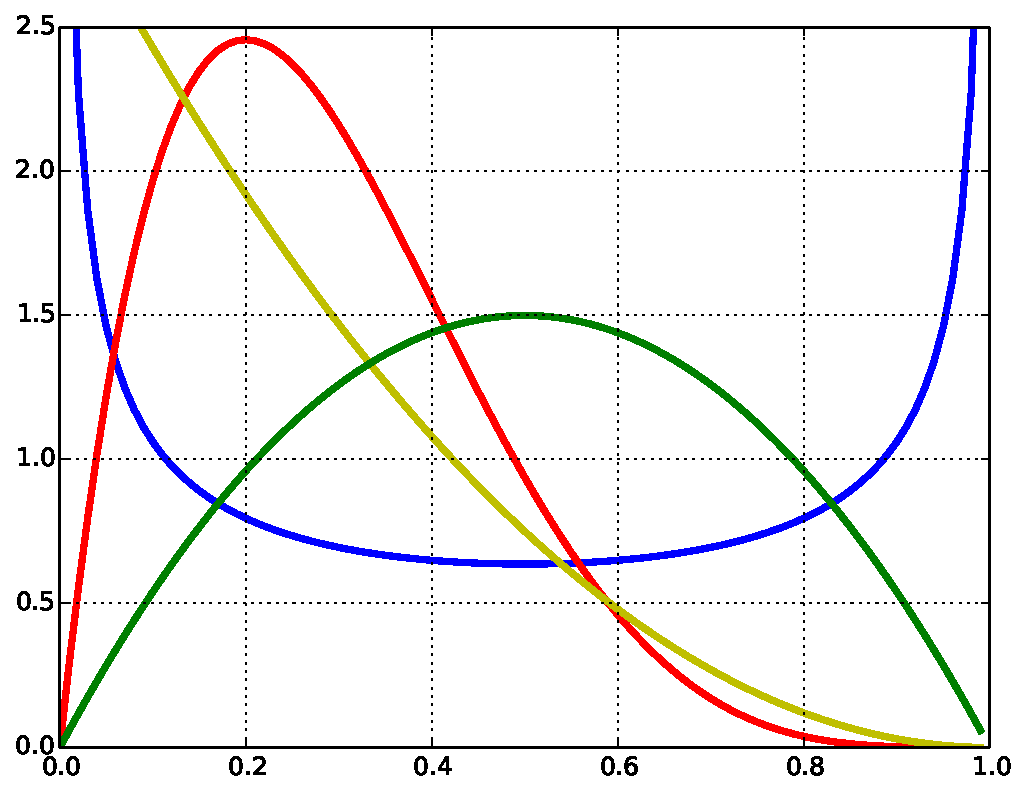
\includegraphics[width=183pt, height=142pt]{img/beta}
 Beta
\end{Figure}
\begin{Figure} \centering
 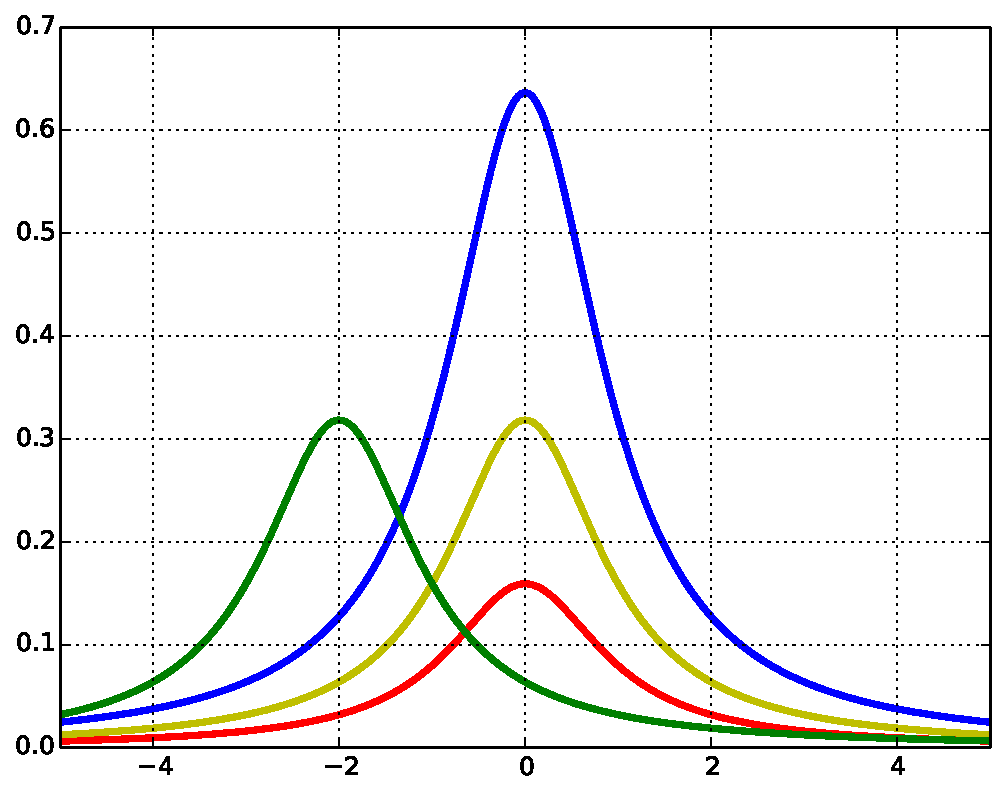
\includegraphics[width=183pt, height=142pt]{img/cauchy}
 Cauchy'ego
\end{Figure}
\begin{Figure} \centering
 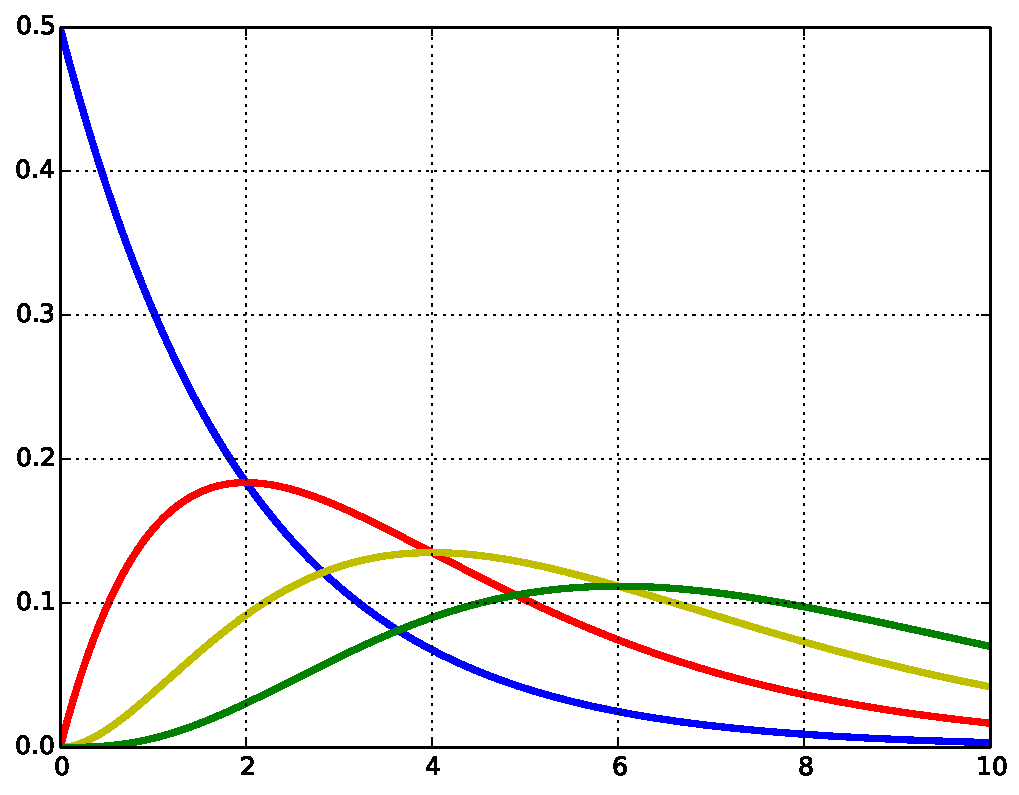
\includegraphics[width=183pt, height=142pt]{img/chi}
 Chi-kwadrat
\end{Figure}
\begin{Figure} \centering
 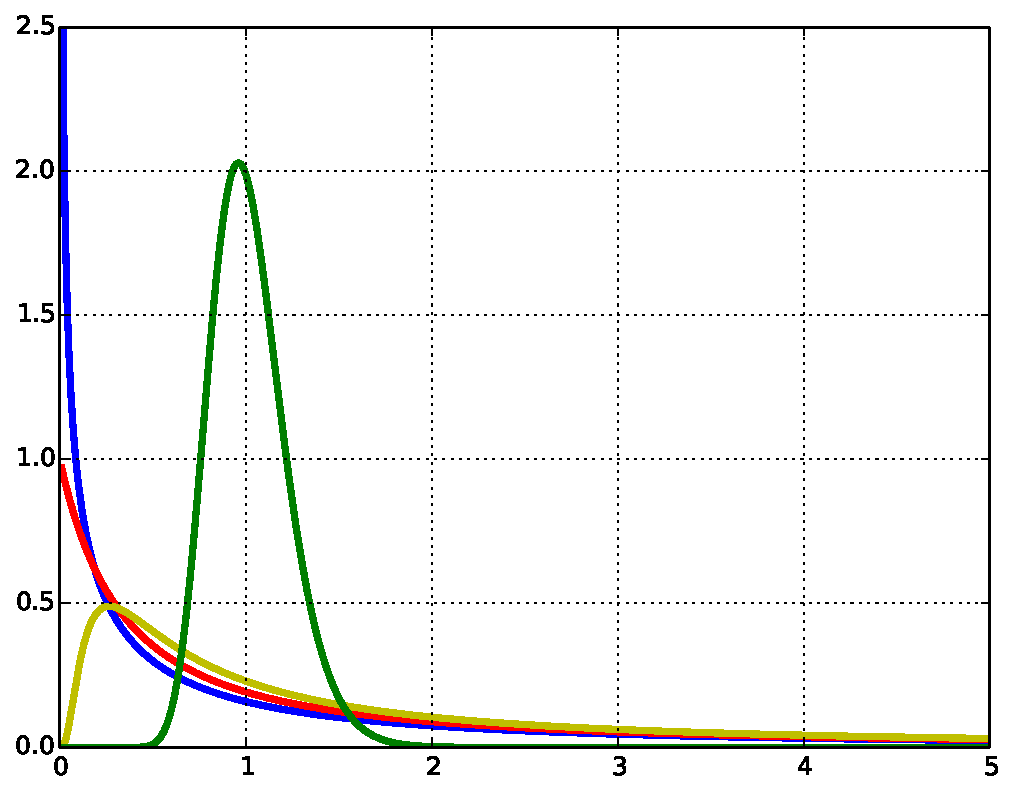
\includegraphics[width=183pt, height=142pt]{img/f}
 F Snedecora
\end{Figure}
\begin{Figure} \centering
 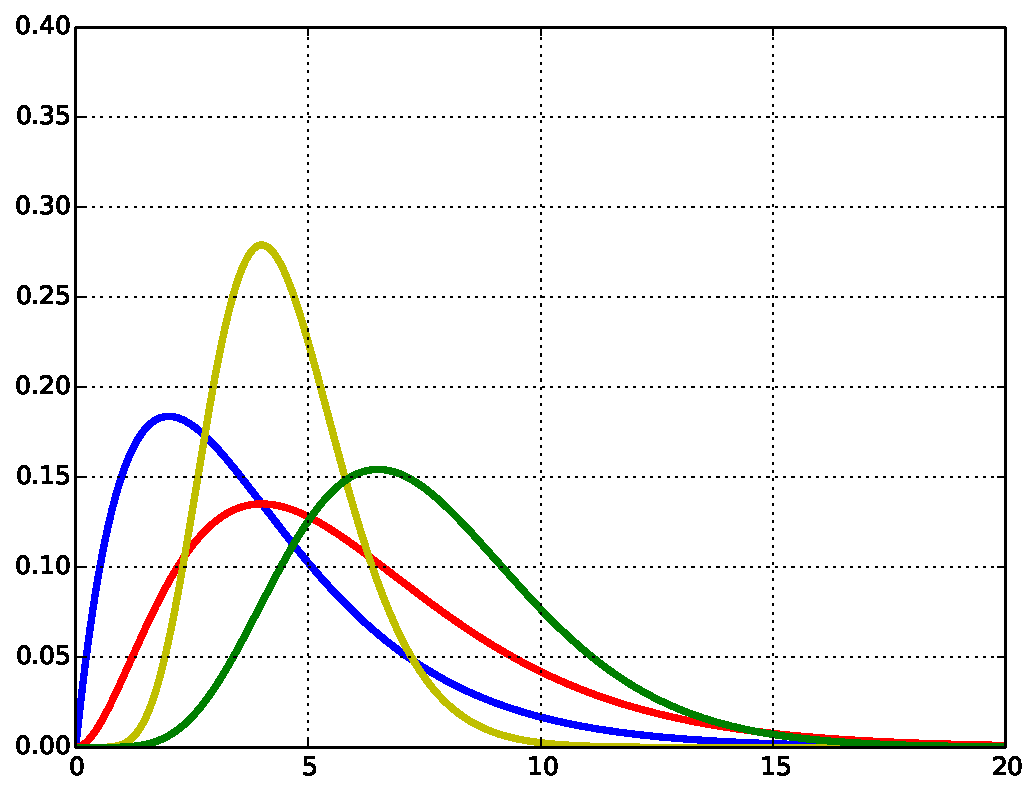
\includegraphics[width=183pt, height=142pt]{img/gamma}
 Gamma
\end{Figure}
\begin{Figure} \centering
 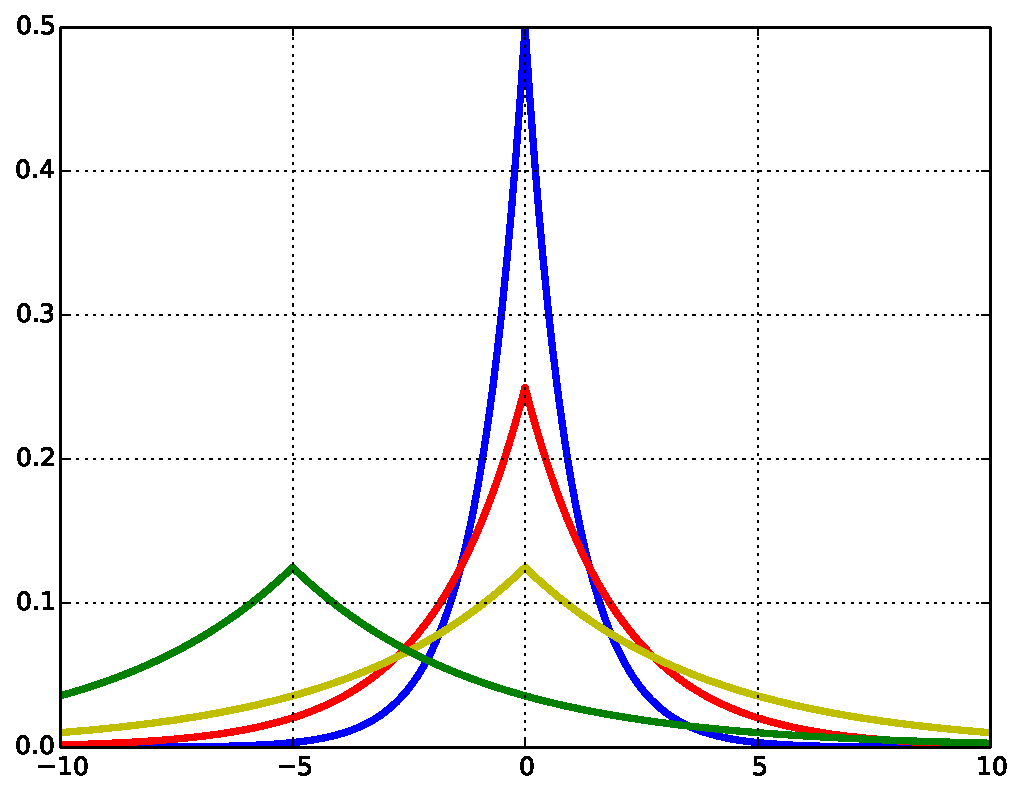
\includegraphics[width=183pt, height=142pt]{img/laplace}
 Dwuwykładniczy Laplace'a
\end{Figure}
\begin{Figure} \centering
 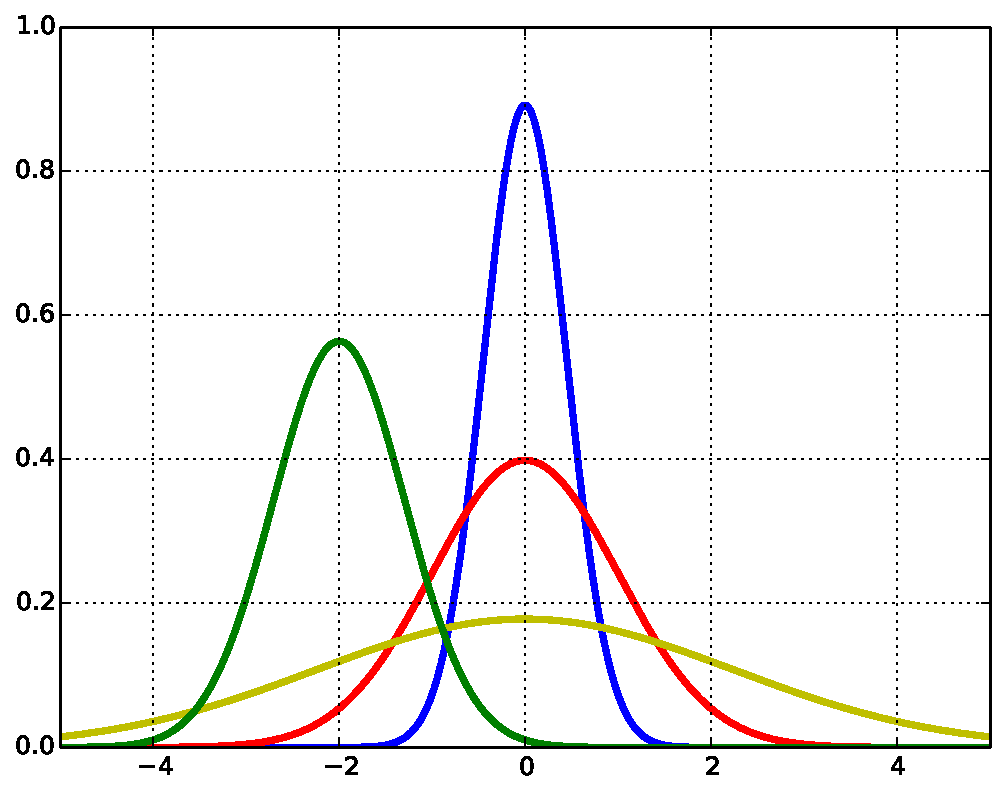
\includegraphics[width=183pt, height=142pt]{img/normalny}
 Normalny
\end{Figure}
\begin{Figure} \centering
 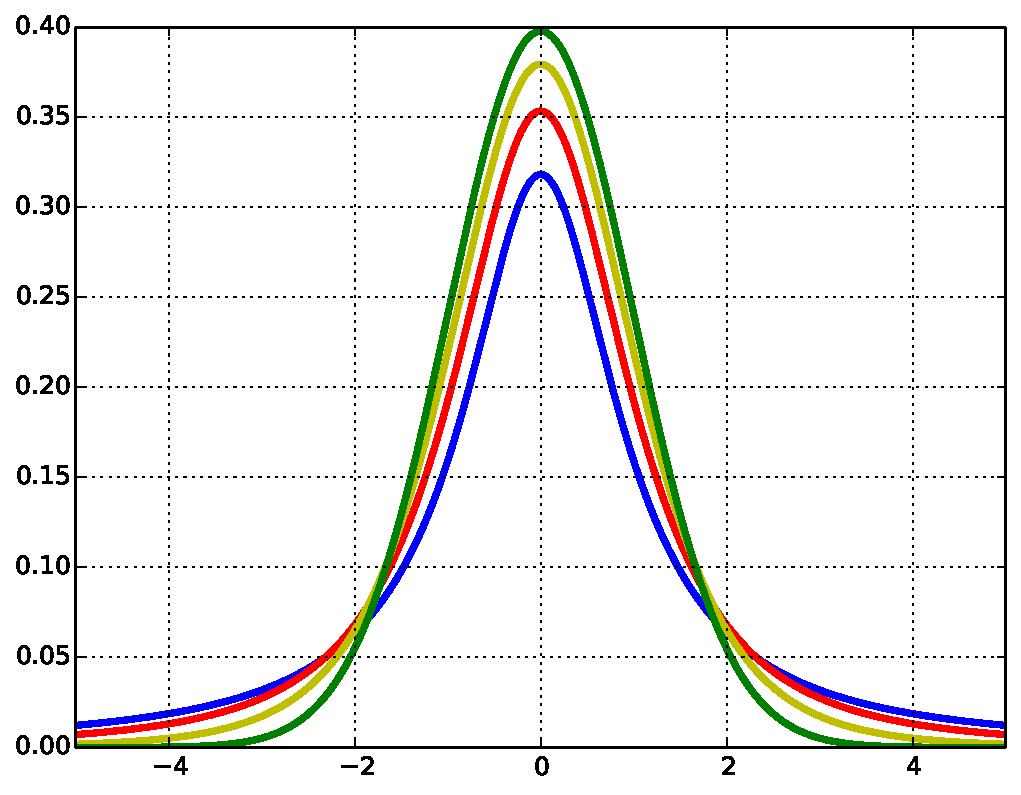
\includegraphics[width=183pt, height=142pt]{img/student}
 t-Studenta
\end{Figure}
\begin{Figure} \centering
 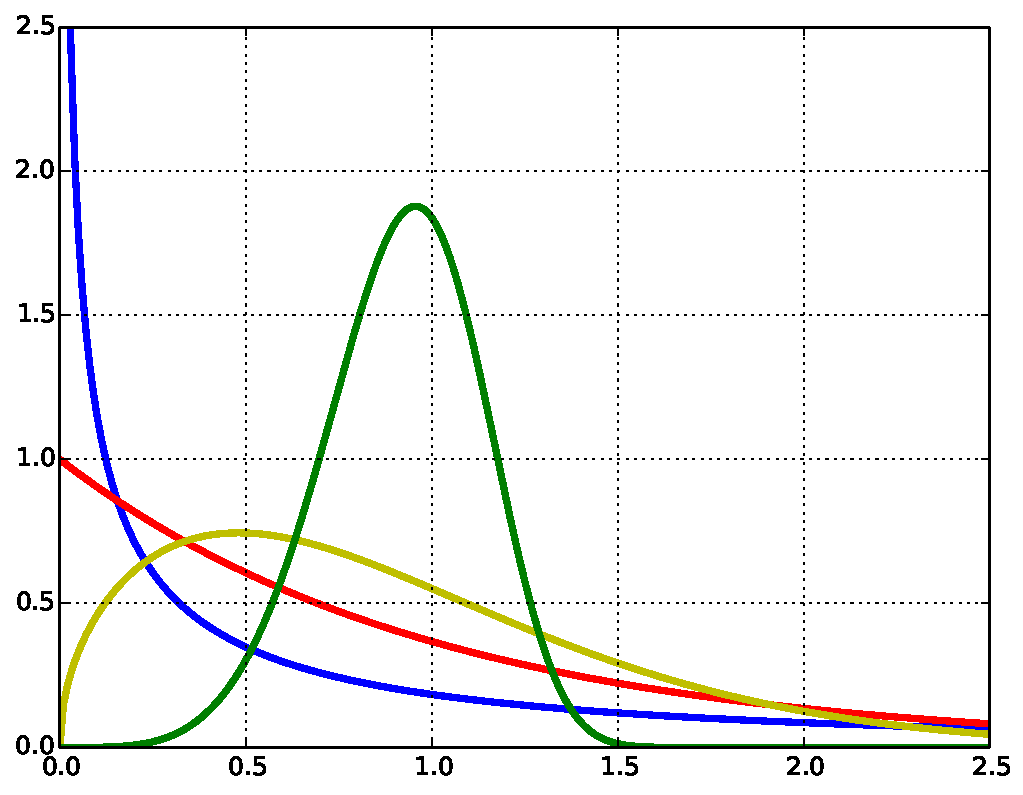
\includegraphics[width=183pt, height=142pt]{img/weibull}
 Weibulla
\end{Figure}
\begin{Figure} \centering
 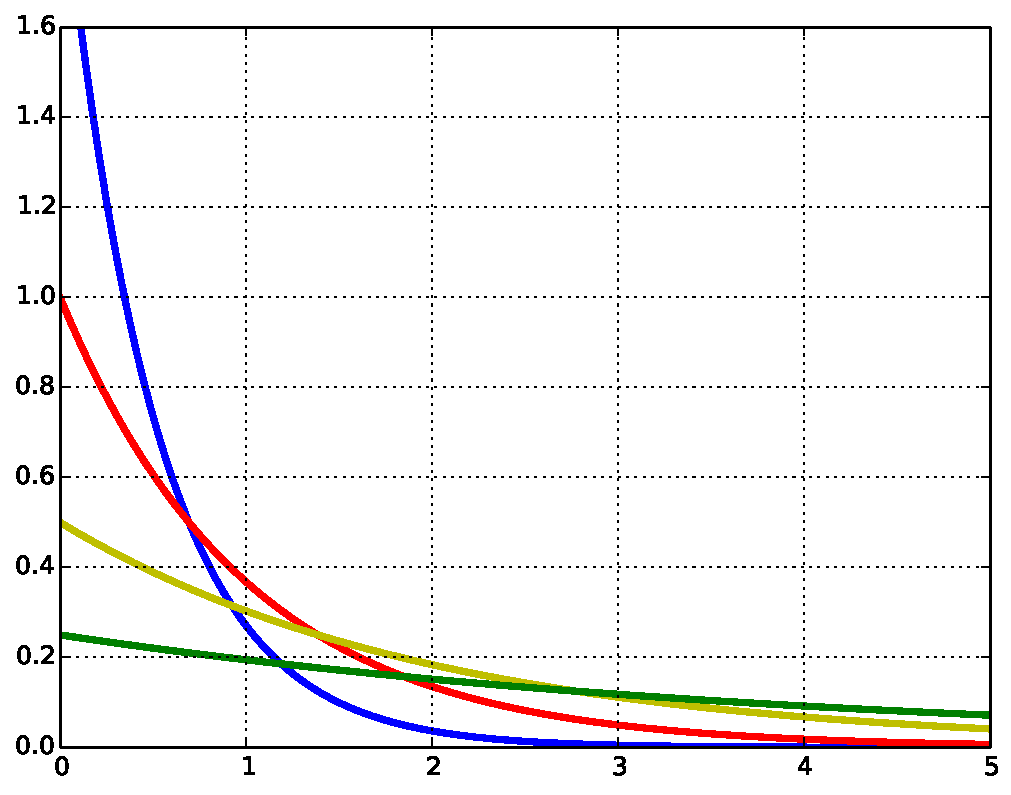
\includegraphics[width=183pt, height=142pt]{img/exp}
 Wykładniczy
\end{Figure}
\begin{Figure} \centering
 
\includegraphics[width=183pt, height=142pt]{img/empty}
 {\color{white}x}
\end{Figure}
\begin{Figure} \centering
 
\includegraphics[width=183pt, height=142pt]{img/empty}
 {\color{white}g}
\end{Figure}
\end{multicols}

\begin{multicols}{2}
\begin{enumx}
\item Beta: $(\alpha, \beta)$ = \textbf{\color{blue}(0.5, 0.5)}, \textbf{\color{red}(2, 5)}, \textbf{\color{zolty}(1, 3)}, \textbf{\color{Green}(2, 2)}.
\item Cauchy'ego: $\gamma$ = \textbf{\color{blue}0.5}, \textbf{\color{red}2}, \textbf{\color{zolty}1} ($x_0 = 0$), \textbf{\color{Green}1} ($x_0 = -2$).
\item Chi-kwadrat: $k$ = \textbf{\color{blue}2}, \textbf{\color{red}4}, \textbf{\color{zolty}6}, \textbf{\color{Green}8}.
\item Snedecora: \textbf{\color{blue}(1, 1)}, \textbf{\color{red}(2, 1)}, \textbf{\color{zolty}(10, 1)}, \textbf{\color{Green}(100, 100)}.
\item Gamma: $(\alpha, \beta)$ = \textbf{{\color{blue}(2, 0.5)}}, \textbf{{\color{red}(3, 0.5)}}, \textbf{\color{zolty}(9, 2)}, \textbf{\color{Green}(7.5, 1)}.
\item Laplace'a: $b = $ \textbf{{\color{blue}1}}, \textbf{{\color{red}2}}, \textbf{\color{zolty}4} ($\mu = 0$), \textbf{\color{Green}4} ($\mu = -5$).
\item Normalny: $\sigma^2$ = \textbf{{\color{blue}0.2}}, \textbf{{\color{red}1.0}}, \textbf{\color{zolty}5.0} (i $\mu = 0$), \textbf{\color{Green}0.5} (i $\mu = -2$).
\item t-Studenta: \textbf{{\color{blue}1}}, \textbf{{\color{red}2}}, \textbf{\color{zolty}5}, \textbf{\color{Green}$\infty$} stopni swobody.
\item Weibull: $\lambda = 1$, $k$ = \textbf{{\color{blue}0.5}}, \textbf{{\color{red}1}}, \textbf{\color{zolty}1.5}, \textbf{\color{Green}5}.
\item Wykładniczy: $\lambda = $, \textbf{{\color{blue}2}}, \textbf{{\color{red}1}}, \textbf{\color{zolty}0.5}, \textbf{\color{Green}0.25}.
\end{enumx}
\end{multicols}
\end{document}

\end{center}



Jednostajny.
Skellam.